% To add an image or include a .tex file you need to add
% \CWD
% to the relative (to the main document) path.
%
% Example:
% \begin{figure}
%   \centering
%   \includegraphics{\CWD/images/example.pdf}
% \end{figure}

O Jogo possui 3 tabuleiros. Em cada tabuleiro, há uma peça e obstáculos. A peça inicialmente está na posição superior esquerda. Em um movimento, um jogador escolhe um dos 3 tabuleiros e move a peça uma quantidade não-nula de espaços para baixo ou para a direita de tal forma que ela não atravesse nem pare em um obstáculo. Jogam dois jogadores alternadamente, quem não tiver movimento, perde.

Você vai jogar O Jogo contra seu amigo. Ele vai começar, mas, logo antes, ele vai passar numa pastelaria para comer um pastel. Você, obviamente, vai roubar. Você vai fazer até um movimento em cada tabuleiro antes dele voltar (seu amigo é esperto, se você fizer mais de um movimento em um tabuleiro ele vai notar).

\begin{figure}[H]
    \centering
    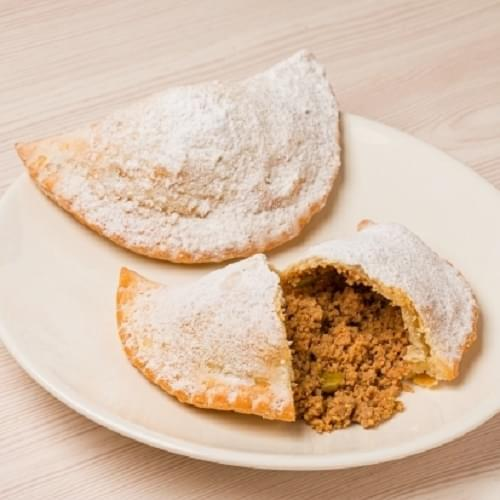
\includegraphics[width=5cm]{\CWD/Pastel-de-Festa.jpg}
  \end{figure}

De quantas formas você pode fazer até um movimento em cada tabuleiro, de tal forma que, quando seu amigo voltar, ao jogar o jogo (ele começa), se ambos jogarem de forma ótima, você ganha?

%
% For input, use one of the following
%

\section*{Entrada}

A entrada consist em três tabuleiros. Cada tabuleiro é representado por uma linha com as dimensões $N$ e $M$ do tabuleiro $1 \leq N\times M \leq 10^5$. Em seguida há $N$ linhas, cada uma com $M$ caracteres: {\tt .} se for uma posição vazia e {\tt x} se for um obstáculo. É garantido que nunca haverá um obstáculo na posição superior esquerda de um tabuleiro.

%
% For output, use one of the following
%

\section*{Saída}

Um único inteiro: o número de formas de se fazer até um movimento em cada um dos três tabuleiros de forma que você ganha O Jogo.

%\sampleio will look for files named sample-n.in and sample-n.sol (where n is 1, 2, 3...)
%in the documents directory and include them as samples.

\section*{Restrições}

\begin{itemize}
\item $1 \leq N\times M \leq 10^5$
\end{itemize}

\exemplo

\bigskip
\textbf{Explicação do Exemplo 1}: Podemos fazer um dos dois movimentos possíveis no segundo tabuleiro; dessa forma, apenas o primeiro tabuleiro tem jogadas possíveis, e podemos ver que o primeiro jogador ganha. Outra possibilidade é fazer um dos dois movimentos no primeiro tabuleiro. Pode ser provado que no arranjo inicial o segundo jogador ganha.

